\documentclass[11pt]{article}
%\usepackage{abbrevs}
\usepackage{natbib}
\usepackage{hyperref}
\usepackage{float}
\usepackage[pdftex]{graphicx}     % could insert ``draft'' between []
\pagestyle{empty}

\setlength{\oddsidemargin}{0pt} % there is 1 inch before the
                                % side margin in ``article'' class
\setlength{\textwidth}{6.5in}

\setlength{\voffset}{0pt}
\setlength{\topmargin}{-0.75in}     % there is 1 inch before the
                                % top margin in ``article'' class and
                                % then room for header, etc.
\setlength{\textheight}{10.0in}
%%%%%%%%%%%

\newcommand{\inch}{$^{\prime\prime}$}
\newcommand{\foot}{$^{\prime}$}
\renewcommand{\deg}{^\circ}

\begin{document}
\title{YOUR TITLE HERE}
%\maketitle

\begin{figure}[H]
\centering
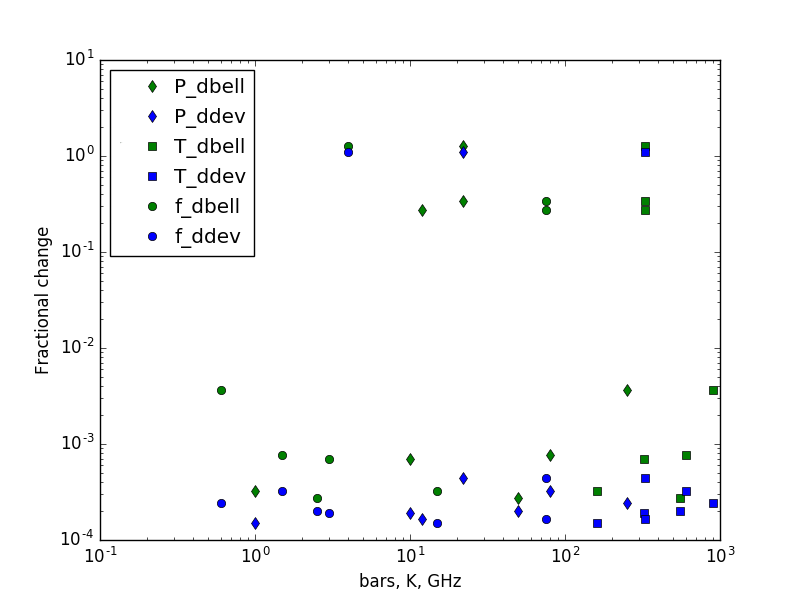
\includegraphics[width=0.75\textwidth]{pc.png}
\caption{Fractional change between Amadeo supplied values and my implementation. \newline ($|$you - me$|$/you)}
\end{figure}

\begin{figure}[H]
\centering
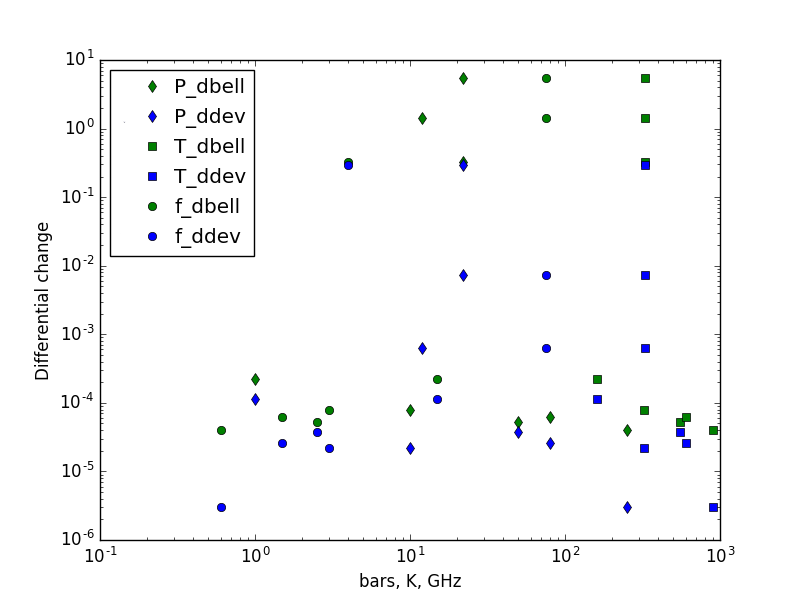
\includegraphics[width=0.75\textwidth]{dc.png}
\caption{Difference between Amadeo supplied values and my implementation.  \newline ($|$you - me$|$)}
\end{figure}

\newpage
These are complicated figures where I plot all parameters (P, T, mixing ratio) as different symbols with Bellotti comparisons as green and Devaraj comparisons as blue.  The bold entries highlight the ones that are different.  Looking at the row for 4 GHz, 22 bars, 330 K, if I change the pressure to 12 bars it matches very well (and perfectly if I swap Bellotti/Devaraj) -- see the entry added to the bottom.  Maybe this was a transcription error?

The only other ones are for high frequencies, so maybe I have the values ``above'' the frequency switch at 30 GHz wrong.  Here are my values:
\begin{verbatim}
    if freq<=30.0:
        gnu_H2=1.6937;      gnu_He=0.6997;       gnu_NH3=0.7523;
        GAMMA_H2=0.8085;    GAMMA_He=1.0;        GAMMA_NH3=1.0;
        zeta_H2=1.3263;     zeta_He=0.1607;      zeta_NH3=0.6162;
        Z_H2=0.8199;        Z_He=-0.7269;        Z_NH3=1.3832;
        d=-0.0139;
        Con=0.9619;
    else:
        gnu_H2=1.7465;      gnu_He=0.9779;      gnu_NH3=0.7298;
        GAMMA_H2=0.8202;    GAMMA_He=1.0;       GAMMA_NH3=1.0;
        zeta_H2=1.2163;     zeta_He=0.0291;     zeta_NH3=0.5152;
        Z_H2=0.8873;        Z_He=0.8994;        Z_NH3=2.0/3.0;
        d=-0.0627;
        Con=0.9862;
\end{verbatim}

\begin{table}
\caption{Values supplied by Amadeo/my implementation of them.  Bold ones are the ones that show significant differences.}
\begin{tabular}{| l | l | l | r | r | r | c | c |} \hline
 {\bf F(GHz)}& {\bf P(bars)}& {\bf T(K)} &  {\bf NH3}  &  {\bf H2}  &  {\bf He}  & {\bf Bellotti NH3 (dB/km)} & {\bf Devaraj NH3 (dB/km)} \\ \hline
 15    & 1      & 160  &  2E-4 & 0.87 & 0.13 &        0.6873/0.6875        &        0.7399/0.7400       \\ \hline
 3     & 10     & 325  &  2E-4 & 0.87 & 0.13 &        0.1150/0.1151        &        0.1136/0.1136       \\ \hline
 2.5   & 50     & 550  &  2E-4 & 0.87 & 0.13 &        0.1922/0.1922        &        0.1902/0.1902       \\ \hline
 1.5   & 80     & 600  &  2E-4 & 0.87 & 0.13 &        0.0802/0.0803        &        0.0813/0.0813       \\ \hline
 75    & 22     & 330  &  2E-4 & 0.87 & 0.13 &        {\bf 16.2537/10.7199}       &        16.7760/16.7686       \\ \hline
 75    & 12     & 330  &  2E-4 & 0.87 & 0.13 &        {\bf 5.1798/3.7548}        &        3.7556/3.7562       \\ \hline
 4     & {\em 22}     & 330  &  2E-4 & 0.87 & 0.13 &        {\bf 0.2562/0.5810}        &        {\bf 0.2645/0.5561}       \\ \hline
 0.6   & 250    & 900  &  2E-4 & 0.87 & 0.13 &        0.0111/0.0111        &        0.0125/0.01250       \\ \hline \hline \hline
 4     & {\em 12}     & 330  &  2E-4 & 0.87 & 0.13 &        {\em 0.2562/0.2645}        &        {\em 0.2645/0.2562}       \\ \hline
\end{tabular}
\end{table}

\bibliographystyle{plainnat}
\bibliography{YOUR BIBLIOGRAPHY HERE}
\end{document}
